%!TEX root = ../AST208-notes.tex

\begin{quote} It's more important to know whether there will be weather than what the weather will be. ---Norton Juster, \emph{The Phantom Tollbooth}\end{quote}

\section{Hydrostatic equilibrium}

Let's consider a fluid at rest in a gravitational field. By \emph{at rest}, we simply mean that the fluid velocity is sufficiently small that we can neglect the inertia of the moving fluid in our equation for force balance.  By a \emph{fluid}, we mean that the pressure is isotropic\sidenote{Meaning the pressure is the same in all directions.} and directed perpendicular to a surface.  Let's now imagine a small fluid element, with thickness $\Delta r$ and cross-sectional area $\Delta A$, as depicted in Fig.~\ref{f.hydrostatic-equilibrium}.
\begin{marginfigure}
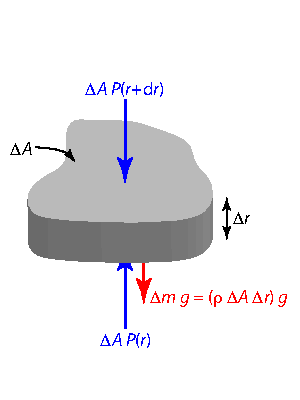
\includegraphics[width=\linewidth]{hydrostatic-equilibrium}
\caption[A fluid element in hydrostatic equilibrium]{A fluid element in hydrostatic equilibrium.
\label{f.hydrostatic-equilibrium}}
\end{marginfigure}

The weight of the fluid element is $\Delta m g$, where $g$ is the gravitational acceleration and $\Delta m =  \Delta A\times\Delta r\times \rho$ is the mass of the fluid element with $\rho$ being the mass density.
The force on the upper face is $\Delta A\times P(r+\Delta r)$; on the lower face, $\Delta A\times P(r)$.  Here $P(r)$ is the pressure.  For the element to be in hydrostatic equilibrium the forces must balance,
\[
	\Delta A \left[ -P(r+\Delta r) + P(r) - \Delta r \rho g  \right] = 0;
\]
dividing by $\Delta r$ and taking the limit $\Delta r \to 0$ gives us the equation of hydrostatic equilibrium:
\begin{equation}\label{e.hydrostatic-equilibrium}
	\DD{P}{r} = -\rho g.
\end{equation}
For an incompressible fluid in constant gravity, the pressure increases linearly with depth. This is a good approximation to the pressure in Earth's oceans.  In general, however, the density $\rho$ depends on the pressure $P$, and we need more information to solve for the atmospheric structure.

\marginnote{The SI unit of pressure is the \textbf{Pascal}: $\val{1}{\unitstyle{Pa}} = \val{1}{\unitstyle{N}\usk\meter^{-2}}$. The mean pressure at terrestrial sea level is $\val{1}{\unitstyle{atm}} = \val{\sci{1.013}{5}}{\unitstyle{Pa}}$. Other common units of pressure are the \textbf{bar} ($\val{1}{\unitstyle{bar}} = \val{10^{5}}{\unitstyle{Pa}}$) and the \textbf{Torr} ($\val{760}{\unitstyle{Torr}} = \val{1}{\unitstyle{atm}}$).}
\begin{exercisebox}[Pressure increase in water]
Water is nearly incompressible and has a density of $\val{10^{3}}{\kilo\gram\usk\meter^{-3}}$.  How deep would you need to dive for the pressure to increase by $\val{1}{\unitstyle{atm}} = \val{\sci{1.013}{5}}{\unitstyle{Pa}}$?  The gravitational acceleration at Earth's surface is $\val{9.8}{\meter\usk\second^{-2}}$.
\end{exercisebox}

Let's look at this in a bit more detail.  Suppose we take our fluid layer to be thin, so that $g$ is approximately constant. Then we can write equation~(\ref{e.hydrostatic-equilibrium}) as
\[ \int_{P_{0}}^{P_(z)} \dif P = -g\int_{0}^{z} \rho\,\dif z. \]
Now consider a cylinder of cross-section $\Delta A$ that extends from $0$ to $z$.  The mass of that cylinder is
\[ m(z) = \Delta A\times\int_{0}^{z}\rho \,\dif z.
\]
and its weight is $m(z)g$.
\begin{marginfigure}
\centering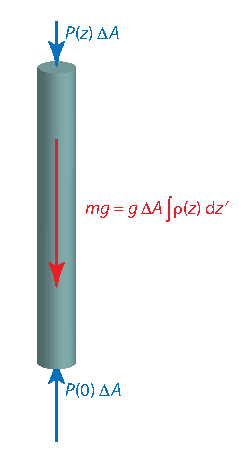
\includegraphics[width=0.8\linewidth]{column}
\caption[The mass of a column of fluid]{
The mass of a column of fluid.
\label{f.column}}
\end{marginfigure}

The difference in pressure between the bottom and top of the cylinder is just
\[ P_{0}-P(z) = g m(z)/\Delta A, \]
that is, the weight per unit area of our column.  Let's apply this to our atmosphere:
if we take the top of our column to infinity and the pressure at the top to zero, then the pressure at the bottom (sea level) is just the weight of a column of atmosphere with a cross-sectional area of $\val{1}{\meter^{2}}$.

\section{The ideal gas}\label{s.ideal-gas}
To solve equation~(\ref{e.hydrostatic-equilibrium}) we need at a minimum a relation between pressure and density. A relation between pressure, density, and temperature is called an \textbf{equation of state}.
For an ideal gas\sidenote[][\baselineskip]{By \emph{ideal} gas, we mean that the particles are non-interacting; as a result, the energy of the gas only depends on the kinetic energy of the particles and in particular is independent of the volume.} of $N$ particles in a volume $V$ at pressure and temperature $P$ and $T$, the equation of state is
\begin{equation}\label{e.ideal-gas-eos}
PV = NkT
\end{equation}
where $k = \val{\sci{1.381}{-23}}{\unitstyle{J}\usk\K^{-1}}$ is \textbf{Boltzmann's constant}.

In chemistry, it is convenient to count the number of particles by \textbf{moles}.  One mole of a gas has $\NA = \sci{6.022}{23}$ particles\sidenote{The constant $\NA$ is known as \textbf{Avogadro's number}.}, and the number of moles in a sample is $n = N/\NA$.  If we divide and multiply equation~(\ref{e.ideal-gas-eos}) by $\NA$, then our ideal gas equation becomes
\[ PV = n\left[\NA k\right]T \equiv n R T, \]
where $R = \NA k = \val{8.314}{\unitstyle{J}\usk\K^{-1}\usk\mol^{-1}}$ is the gas constant. This is perhaps the most familiar form of the ideal gas law---but it is not in a form useful to astronomers.

We astronomers don't care about little beakers of fluid---we have whole worlds to model! Let's take our ideal gas law and introduce the molar weight $m$ as the mass of one mole of our gas.  Then the ideal gas law can be written
\begin{equation}\label{e.ideal-gas-astro}
 P = \left(\frac{mN/\NA}{V}\right)\frac{k\NA}{m} T \equiv \rho \frac{k\NA}{m} T.
\end{equation}
The quantity in parenthesis is the mass per volume, or density $\rho$, of our fluid.  This is the same mass density that appears in equation~(\ref{e.hydrostatic-equilibrium}).  Equation~(\ref{e.ideal-gas-astro}) is the form most convenient for fluid dynamics, because it is in terms of intrinsic fluid properties rather than in terms of a laboratory quantity like volume.

\section{The scale height}\label{s.scale-height}
Let's take a first stab at modeling Earth's atmosphere with equation~(\ref{e.hydrostatic-equilibrium}). We'll take Earth's atmosphere to be an ideal gas and for simplicity we'll assume the temperature doesn't change with altitude\sidenote[][-\baselineskip]{This isn't true, of course, but let's keep things simple and see how we do.}  The molar weight of dry\sidenote[][\baselineskip]{The water vapor content of air varies considerably depending on ambient conditions.} air is $\val{0.02897}{\kilo\gram\usk\mol^{-1}}$.  Using equation~(\ref{e.ideal-gas-astro}) to eliminate $\rho$ in equation~(\ref{e.hydrostatic-equilibrium}), we obtain
\[
	\frac{1}{P}\DD{P}{z} = -\frac{mg}{\NA kT},\quad\textrm{or} \quad\frac{\dif P}{P} = -\frac{mg}{\NA kT}\,\dif z.
\]
Integrating from $z=0$, where $P(z=0)=P_{0}$, to a height $z$ gives us an equation for the pressure as a function of height,
\begin{equation}\label{e.exp-atm}
	P(z) = P_{0}\exp\left[-\frac{mgz}{\NA kT}\right].
\end{equation}
Since the argument of the exponential is dimensionless, we see that we can write $P(z) = P_{0}e^{-z/H_{P}}$, where
\[  H_{P} = \frac{\NA kT}{mg} \]
is the \textbf{pressure scale height}---the height over which the pressure decreases by a factor $1/e$.

\begin{exercisebox}[Scale height for dry air]
Evaluate $H_{P}$ for dry air at a temperature of $\val{288}{\K}$ ($\val{15}{^{\circ}\unitstyle{C}}$).  Check that your answer is reasonable based on your experience.  In fact, this value of $H_{P}$ is overly large because the temperature in the troposphere does, in fact, decrease with height at an average \textbf{lapse rate} of
\[
	\DD{T}{z} = -\val{6.5}{^{\circ}\unitstyle{C}\usk\kilo\meter^{-1}}.
\]
\end{exercisebox}

\section{The adiabatic thermal gradient}\label{s.adiabatic-gradient}
Hot air rises. This simple phenomenon sets the lapse rate in the troposphere. Warm surface air rises quickly enough that there is little exchange of heat with colder, downward moving air.  As a result, the fluid motions are \textbf{adiabatic}.  To understand what this means, recall the first law of thermodynamics\cite{Fermi1956Thermodynamics}, which relates the change in internal energy $\dif U$ and in volume $\dif V$ to the heat transferred $\dif Q$:
\begin{equation}\label{e.first-law-thermo}
	\dif Q = \dif U + P\dif V,
\end{equation}
where $P$ is the pressure.  Now, we aren't using volume to describe our fluid\sidenote{cf.\ eq.~(\ref{e.ideal-gas-astro})} so let's apply this equation to $\val{1}{\mol}$ of our fluid, and divide both sides by the molar mass $m$.  Then $Q$ refers to the heat transferred \emph{per kilogram}, and $U$ refers to the internal energy \emph{per kilogram}.  Instead of $\dif V$, we then have $\dif V/(\val{1}{\mol}\times m) = \dif(1/\rho) = -\rho^{-2}\dif\rho$.  Our first law, rewritten in terms of mass-specific quantities, is thus
\begin{equation}\label{e.first-law-thermo-astro}
	\dif Q = \dif U -\frac{P}{\rho^{2}}\dif \rho.
\end{equation}
Suppose we wish to express quantities in terms of temperature $T$ and density $\rho$: then
\[ \dif U = \tderiv{U}{T}{\rho}\dif T + \tderiv{U}{\rho}{T}\dif \rho, \]
and
\[ \dif Q = \tderiv{U}{T}{\rho}\dif T + \left[\tderiv{U}{\rho}{T} - \frac{P}{\rho^{2}}\right]\dif \rho. \]
Hence the heat needed to raise the temperature of one kilogram of fluid when holding density fixed is
\begin{equation}\label{e.CV}
C_{\rho} \equiv \tderiv{Q}{T}{\rho} = \tderiv{U}{T}{\rho}.
\end{equation}
For an ideal gas, $U = U(T)$ and $C_{\rho}$ is approximately constant; hence we may integrate equation~(\ref{e.CV}) to obtain $U = C_{\rho}T + \textrm{const.}$.

In Eq.~(\ref{e.first-law-thermo-astro}), the last term is $-(P/\rho)\, \dif\rho/\rho = -(P/\rho)\,\dif\ln\rho$. This illustrates a useful trick: take the logarithm of the equation of state, $\ln (P) = \ln(\rho) + \ln (T) + \ln (k\NA/m)$, and then take the differential to obtain
\[ \frac{\dif P}{P} = \frac{\dif\rho}{\rho} + \frac{\dif T}{T}. \]
Now eliminate $\dif\rho/\rho$ in the equation
\[ \dif Q = C_{\rho}\dif T - \frac{P}{\rho}\frac{\dif\rho}{\rho} \]
to obtain an expression for the heat transferred as a function of temperature and pressure,
\[ \dif Q = \left[C_{\rho} + \frac{P}{\rho T}\right]\dif T - \frac{1}{\rho}\dif P
	 = \left[C_{\rho} + \frac{k\NA}{m}\right]\dif T - \frac{1}{\rho}\dif P. \]
From this we see that the heat needed to raise the temperature of one mole when holding pressure fixed is
\begin{equation}\label{e.CP}
C_{P}\equiv \tderiv{Q}{T}{P} = C_{V} + \frac{k\NA}{m}.
\end{equation}
The specific heat of one mole of various ideal gases is given in Table~\ref{t.specific-heat}.
\begin{table}
\caption{Specific heats for ideal gases.\label{t.specific-heat}}
\begin{tabular}{lrrr}
gas & $C_{\rho}$ & $C_{P}=C_{\rho}+k\NA/m$ & $\gamma = C_{P}/C_{\rho}$\\
\hline
monatomic & $(3/2) k\NA/m$ & $(5/2)k\NA/m$ & $5/3$\\
diatomic & $(5/2) k\NA/m$ & $(7/2)k\NA/m$ & $7/5$\\
\end{tabular}
\end{table}
It is important to remember that these relations for the specific heats are for an ideal gas and are not universally true.

\newthought{During convection, hot air rises and cool air descends, and both move adiabatically.}  By adiabatically, we mean that there is no heat exchange:
\[ 0 = \dif Q = C_{P}\dif T - \frac{1}{\rho} \dif P.\]
Using the ideal gas equation of state we can eliminate $\frac{1}{\rho} = (k\NA/m) T/P$ and write
\[ \frac{\dif T}{T} = \frac{k\NA}{mC_{P}} \frac{\dif P}{P} = \frac{C_{P}-C_{V}}{C_{P}} \frac{\dif P}{P} = \frac{\gamma-1}{\gamma}\frac{\dif P}{P}. \]
Integrating both sides of the equation gives
\[ \ln T = \frac{\gamma-1}{\gamma}\ln P + \textrm{const.},\]
or 
\begin{equation}\label{e.adiabat}
 T = T_{0}\left(\frac{P}{P_{0}}\right)^{(\gamma-1)/\gamma},
\end{equation}
where $T_{0}$ and $P_{0}$ are the temperature and pressure at the beginning of the adiabatic process.
Equation~(\ref{e.adiabat}) tells us how the temperature changes with pressure along an adiabat for an ideal gas.

\begin{exercisebox}[Adiabatic lapse rate]
Use equations~(\ref{e.adiabat}) and (\ref{e.hydrostatic-equilibrium}) to compute the lapse rate $\dif T/\dif z$ at sea level.  Dry air is composed of mostly diatomic gases with a molar weight $\val{0.02897}{\kilo\gram\usk\mol^{-1}}$. You should find an answer around $\val{-10}{^{\circ}\unitstyle{C}/\kilo\meter}$, which is almost twice as large as the value quoted earlier.  Can you guess why the value you calculated might be off? (\emph{Hint: there is a process we haven't yet accounted for.  If you want a hint, go outside and look up.})
\end{exercisebox}

\section{Atmospheric circulation on a rotating Earth}\label{s.motion-in-atmosphere}

The Sun heats the Earth unevenly; this in turn creates pressure gradients that drive a circulation of the atmosphere and a transfer for heat from the equator polewards.  The Coriolis force deflects the horizontal motion of the air, and this sets up large-scale features in the atmosphere.

Because of the Earth's rotation, in the frame of a particular location on Earth there is both a Coriolis and a centrifugal acceleration:
\begin{eqnarray}
\textrm{Coriolis} &\quad& \bvec{a}_{\mathrm{Cor}} = -2\bvec{\Omega}\vcross\bvec{v}\\
\textrm{centrifugal} &\quad& \bvec{a}_{\mathrm{cen}} = -\bvec{\Omega}\vcross\left(\bvec{\Omega}\vcross\bvec{R}\right)
\end{eqnarray}
where $\bvec{R}$ is the location of our particle and $\bvec{\Omega}$ is the rotation vector of the Earth.  

The centrifugal component just depends on the latitude $\lambda$ and causes the Earth to bulge at the equator to compensate. It doesn't, however, change the motion of air currents.  The vertical component of the Coriolis acceleration will be quite small compared to $\bvec{g}$, so we can neglect it as well. For the horizontal component, if we are at latitude $\lambda$,
\begin{marginfigure}
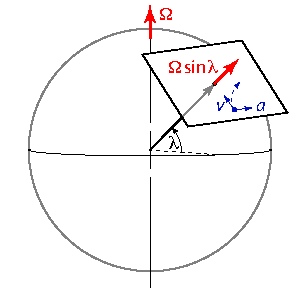
\includegraphics[width=\linewidth]{beta-plane}
\caption{Motion in a horizontal layer in a small region at latitude $\lambda$.}
\end{marginfigure}
\[
a_{\mathrm{Cor}} =  2\Omega v \sin\lambda.
\]
This acceleration is to the right in the northern hemisphere and to the left in the southern.  At the equator it vanishes.

\begin{exercisebox}[Coriolis vs.\ centripetal acceleration around a river bend]
Suppose we have a river flowing at $\val{3}{\kilo\meter/\hour}$.  At our latitude, how does the Coriolis acceleration compare to the centripetal acceleration if the river has a bend with radius of curvature $r$?  How large would $r$ need to be for the Coriolis force to dominate?
\end{exercisebox}

In addition to the Coriolis acceleration from the Earth rotation, horizontal pressure gradients will also produce an acceleration
\[
	-\frac{1}{\rho}\grad P.
\]
A typical horizontal gradient for a weather system is about $\val{0.03}{\milli\unitstyle{bar}/\kilo\meter}$.\marginnote{Recall that $\val{1}{\unitstyle{bar}} = \val{\sci{1.013}{5}}{\unitstyle{Pa}}$.  The density of air at sea level is $\val{1.3}{\kilo\gram\usk\meter^{-3}}$.} Consider a \textbf{cyclone} in which the winds swirl counterclockwise about a low.  Let's look at a small parcel of fluid a distance $r$ from the center of the cyclone, which has a height $H$. The mass of our fluid parcel is $\Delta S\,\Delta r\,H\,\rho$, and the acceleration of the fluid is $-v^{2}/r\,\hat{r}$. The equation for force and acceleration along $\hat{r}$ is therefore
\begin{marginfigure}
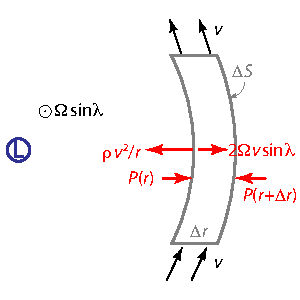
\includegraphics[width=\linewidth]{cyclone}
\caption{Forces on a parcel of air circulating about a low.
\label{f.cyclone}}
\end{marginfigure}
\[
	\left[P(r)-P(r+\Delta r)\right]\Delta S\,H + 2\Delta S\,\Delta r\,H\,\rho\,\Omega v\sin\lambda = -\Delta S\,\Delta r\,H\,\rho \frac{v^{2}}{r}.
\]
or
\begin{equation}\label{e.force-balance}
	\underbrace{\frac{v^{2}}{r}}_{\textrm{centripetal}} 
	+ \underbrace{2 v\Omega\sin\lambda}_{\mathrm{Coriolis}} 
	- \underbrace{\frac{1}{\rho}\DD{P}{r}}_{\mathrm{pressure}} = 0.
\end{equation}

\begin{exercisebox}[Scale of mid-latitude weather systems]
\begin{enumerate}
\renewcommand{\theenumi}{\alph{enumi}}
\renewcommand{\labelenumi}{\alph{enumi})}
\item\label{v-wind}
When $r$ is sufficiently large, we can neglect the centripetal term in equation~(\ref{e.force-balance}).  In that case, for a pressure gradient of $\val{3}{\milli\unitstyle{bar}}/\val{100}{\kilo\meter}$, what is a velocity satisfying this equation. Does this seem realistic?

\item Using the velocity you found in part \ref{v-wind}, determine the size $r$ of the weather system at which the centripetal term becomes comparable to the Coriolis term.
\end{enumerate}
\end{exercisebox}

In tropical regions the latent heat released from condensing water vapor in rising updrafts can produce a strong pressure gradient around a low---a tropical depression. If the pressure gradient is strong enough, a hurricane forms. In this case the pressure gradient can be as strong as $\val{0.3}{\milli\unitstyle{bar}/\kilo\meter}$, and the centripetal term cannot be neglected.
If we consider a hurricane located at  latitude $\lambda=20^{\circ}$ and take the eye region to have $r = \val{100}{\kilo\meter}$, then solving equation~(\ref{e.force-balance}) gives
\[
	v = -r\Omega\sin\lambda + \sqrt{(r\Omega\sin\lambda)^{2}+\frac{r}{\rho}\DD{P}{r}}\approx \val{46}{\meter/\second},
\]
which is typical of hurricane-strength winds.

\begin{exercisebox}[Why the strongest storms are associated with low-pressure systems]
You may have wondered why the strongest storms are associated with low-pressure systems. Repeat the analysis leading to equation~(\ref{e.force-balance}) for air circulating in an anti-cyclone around a pressure high. There is one crucial difference in the equation which leads to a limitation on the pressure gradient and velocities in this case; explain this difference.
\end{exercisebox}
